\chapter{Background}
\label{chapter:background}

\section{Cryptography}

Delfs et.al.~\cite{delfs2007} state that electronic communication has grown rapidly. They further discuss that this expansion has led to increased requirements on digital confidentiality - keeping data safe from manipulation and prying eyes. Although just a part of the vast field of cryptology, cryptography studies the act of keeping information safe - encrypting it on one end and decrypting it on another. As outlined in~\cite{bernstein2017}, cryptographic functions are sorted into two categories - \textit{symmetric-key} functions and \textit{public-key} functions, both of which refer to how the keys to the data are used.

In this section, symmetric-key, public-key and related topics will be further discussed to provide an overview of cryptography.

\subsection{Symmetric-Key Cryptography}

Symmetric-key cryptography is where the same key is shared between both parties and used for both encryption and decryption~\cite{bernstein2017}. Symmetric functions can, besides providing confidentiality, also be used to provide authenticity. If only two parties know of the secret key, one of them may request the other to prove possession of it.

A potential problem when using a symmetric key is the fact that the two parties have to somehow securely exchanged a secret key~\cite{delfs2007}. It is not a trivial task to exchange the keys securely, as anyone may intercept their communication channel. There are many ways of securely exchanging a symmetric key by relying on public-key cryptography.

\subsection{Public-Key Cryptography}
\label{section:background:public-key-cryptography}

Rivest et.al.~\cite{rsa1977} describe the functions of a public-key cryptosystem as follows. Let $E_A$ be an encryption algorithm created by party $A$, \gls{alice}, known by the public. Let $D_A$ be a decryption algorithm created and kept secret by \gls{alice}. Then, a public-key cryptosystem can be described as $D_A(E_A(M))=M$ for any message $M$. Such a cryptosystem must be efficiently computable. Furthermore, it is assumed that \gls{alice} does not compromise $D_A$ by revealing $E_A$.

In~\cite{rsa1977} it is further described that whenever a party $B$, \gls{bob}, wants to send a confidential message $M$ to \gls{alice}, they use \gls{alice}'s public encryption algorithm and send the ciphertext $C$ received from $C=E_A(M)$ to \gls{alice}. On the receiving end, \gls{alice} may access the plaintext message $M$ by decrypting the ciphertext, $M=D_A(C)$~\cite{rsa1977}.

For the cryptosystem to be considered secure, it must be computationally unfeasible for an evil party, \gls{eve}, to efficiently compute $D_A$ from information found in $E_A$~\cite{rsa1977}. A trivial, but inefficient way of deciphering a ciphertext $C$ is to enumerate all possible messages $M$ until $E_A(M)=C$.

In practice, each party is in possession of two keys - a public key and a private key~\cite{bernstein2017}. The public key is known to everyone. The private key only to the party in ownership of the keys. Anyone may encrypt a message using a party's public key, but only the owner of the private key may decrypt the contents. By using the private key to encrypt data, anyone with the public key may decrypt it. This mechanism provides a way to digitally sign a message and can be used to authenticate a party.

\subsection{Key Establishment}

A key establishment protocol, sometimes referred to as a \acrfull{kex}, is a process in which two or more parties securely exchange a shared symmetric key known only to them~\cite{boyd2020}. Such a protocol should be able to be performed securely over an untrusted communication channel.

One class of key establishments protocols is the key transport protocols. A key transport protocol is a protocol where one party generates a shared key which is then securely transferred to one or more parties~\cite{boyd2020}.

In another class of protocols, the key agreement protocols, the parties jointly influence the outcome of the shared key by deriving the key from information supplied by the involved parties. This should be performed in such a way that no single party can predetermine the resulting shared key on their own~\cite{boyd2020}.

\subsection{Key Encapsulation Mechanism}

A \acrfull{kem} is a form of key transport protocol designed to generate a new random shared key. The key is encapsulated in a form which can only be unpacked by the chosen recipient. \glspl{kem} are often more efficient than general encryption schemes and are therefore used in many key establishment designs~\cite{boyd2020}. A \gls{kem} consists of four sets and three algorithms~\cite{boyd2020}, listed below.

\begin{itemize}
    \item $K_E$ - a set of public keys for encryption.
    \item $K_D$ - a set of private keys for decryption.
    \item $R$ - a randomness set.
    \item $C$ - a ciphertext set.
\end{itemize}

\begin{itemize}
    \item A key generation algorithm which outputs a valid public key $K\in K_E$, as well as a private key $K^{-1}\in K_D$.
    \item $(c,k)=\text{Encapsulate}_K()$ - an encapsulation algorithm which takes a public key $K$ and outputs a new symmetric key $k$ as well as the corresponding ciphertext $c\in C$.
    \item $k=\text{Decapsulate}_{K^{-1}}(c)$ - a decapsulation algorithm which takes a private key $K^{-1}$ and a ciphertext $c$ and produces the same symmetric key $k$ as received from the encapsulation algorithm.
\end{itemize}

\noindent To further restrict the definition, we require that if $(c,k)$ is output by the encapsulation function $\text{Encapsulate}_K()$, then $k$ must be output by the corresponding decapsulation function $\text{Decapsulate}_{K^{-1}}(c)$~\cite{boyd2020}.

Although the notation used in the listing above does not respect the chosen randomness set, \glspl{kem} in practice often rely on the use of randomness so that a different $(c,k)$ is returned for each invocation of $\text{Encapsulate}_K()$~\cite{boyd2020}. 

\subsection{Forward Secrecy}

Forward Secrecy is a term used to describe the security of session keys after one or more long-term keys have been exposed~\cite{boyd2020}. A key establishment protocol is said to provide forward secrecy if the compromise of long-term keys does not compromise any previously exchanged session key.

Key agreement protocols may provide forward secrecy if the long-term keys are only used for authentication of the exchange~\cite{boyd2020}. Another way to provide forward secrecy is to use ephemeral keys - keys that are only used for a single run of a key establishment protocol.

\section{Classical Cryptography}
\label{section:background:classical-cryptography}

Classical cryptography is cryptography in use on classical computers such as consumer PCs, smart phones and cloud servers. In classical cryptography, several algorithms based on \gls{rsa} and \gls{ecc} are used for key exchange.

This section will further describe cryptographic systems in use to keep data confidential from attacks run on classical hardware, as well as the threats they face.

\subsection{Applications}
\label{section:background:classical-cryptography:applications}

In \acrfull{tls}, key establishment is used to let parties establish a shared symmetric key~\cite{bernstein2017}. Digital signatures are used to ensure the authenticity of the public keys used in the key establishment. The rest of the communication is secured using symmetric cryptography. \gls{tls} may use any of a wide variety of different key establishment algorithms. Some of these algorithms and parameter sets are recommended for use in a pre-quantum era by organizations such as \gls{nist} and the \gls{ietf}, namely \gls{x25519}~\cite{rfc7748}, \gls{ecdhe}~\cite{nist2019} and \gls{dhe}~\cite{nist2019}.

The elliptic-curve-based \gls{x25519} is used for key exchange in the \gls{vpn} Wireguard~\cite{wireguard2020}. The algorithm uses the \gls{curve25519} curve~\cite{rfc7748}. In some contexts, the \gls{x25519} algorithm is known by the name of the curve~\cite{25519naming}. 

In \gls{tls}, \gls{ecdh}, \gls{ecdhe}, \gls{dh} and \gls{dhe} are used to exchange session keys~\cite{rfc8446}. Other protocols such as SSH also use the same algorithms for key exchange~\cite{williams2011}. Some \glspl{vpn} such as OpenVPN~\cite{openvpn} and IPSec~\cite{rfc2409} also use the same algorithms. Variants of the mentioned key exchange algorithms are also used in messaging applications such as the Signal protocol~\cite{gordon2017}.

\subsection{RSA}

In 1977, L. Rivest et. al.~\cite{rsa1977} wrote a paper on digital signatures and public-key cryptosystems. In the paper they introduced a public-key cryptosystem based on powers and modulo operations. In the system, \gls{alice} first decides on two different primes $p$ and $q$ as well as an integer $s$ which is relatively prime to $(p-1)(q-1)$. \gls{alice} makes $r=p*q$ and $s$ public, but keeps $r$ and $q$ secret. As seen in section \ref{section:background:public-key-cryptography}, the encryption function in a public-key cryptosystem is defined as $E_A(M)$. In \gls{rsa}, the function $E_A$ is defined as $E_A(M)=M^s\;(mod\;r)$, for any message $M$.

The decryption function is defined as $D_A(C)=C^t\;(mod\;r)$ where $t$ is solved from $s*t=1\;(mod\;\phi(r))$~\cite{rsa1977}. The value $\phi(r)$ is the so called Euler totient function, which produces the number of positive integers less than $r$ which are relatively prime to $r$.

The security of the cryptosystem is based on the mathematical problem of factorizing a composite prime~\cite{rsa1977}. That is, under the assumption that it is difficult to factorize a number $n=p*q$ into its factors $p$ and $q$, the system is considered secure.

\subsection{Elliptic Curve Cryptography}

Elliptic curve cryptography is a type of cryptosystems built on finite fields~\cite{delfs2007}. Its security lies in the assumption that solving the discrete logarithm problem in the multiplicative $\mathbb{Z}_p^*$ of a finite field $\mathbb{Z}_p$ is unfeasible.

Elliptic curves generally yield much more dense ciphertexts and requires smaller keys to use when compared to \gls{rsa}, without sacrificing security~\cite{delfs2007}. Implementations are often very fast and outperform comparable \gls{rsa} implementations.

To use an elliptic curve for cryptography, one must establish the following domain parameters~\cite{delfs2007}.

\begin{itemize}
    \item $\mathbb{F}_q$ - the finite base field
    \item $a,b\in\mathbb{F}_q$ - the parameters of the curve $E$
    \item $Q,n$ - the base point $Q\in E(\mathbb{F}_q)$, whose order is a large prime number $n$
    \item $h$ - the cofactor defined by $hn=|E(\mathbb{F}_q)|$
\end{itemize}

\noindent The domain parameters $a,b\in\mathbb{F}_q$ describe the curve $E$ as $y^2=x^3+ax+b$. Illustrations of these curves may be seen in figure \ref{figure:background:elliptic-curves}. Not all curves are suitable for elliptic-curve cryptography, which has led to some being standardized for mass usage~\cite{nist2018}.

\begin{figure}[t]
    \centering
    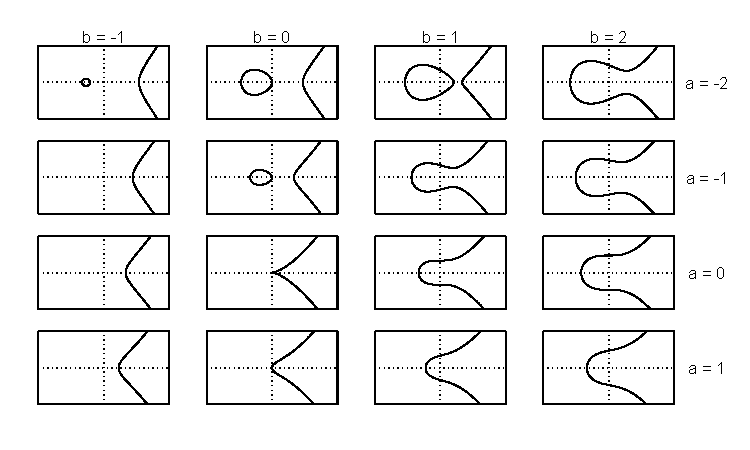
\includegraphics{chapters/background/figures/elliptic-curves.pdf}
    \caption{Illustrations of $y^2=x^3+ax+b$ for various values for $a$ and $b$}
    \label{figure:background:elliptic-curves}
\end{figure}

Elliptic curves are used to replace the multiplicative subgroup $\mathbb{Z}_p^*$ in other cryptosystems based on discrete logarithms, such as \gls{elgamal} and \gls{dsa}~\cite{delfs2007}. The key difference is that elliptic curves define the group operation as $(P, Q)\to P+Q\in E(\mathbb{F}_q)$ for some curve $E$ and two points on the curve $P$ and $Q$ - that is, the group operation of two points on the curve will result in another point on the curve.

\subsection{Diffie-Hellman}
\label{section:background:diffie-hellman}

The \gls{dh} \gls{kex} is a key establishment protocol conceived by Ralph Merkle and published in 1978~\cite{merkle1978}. The work was centered around a novel idea, that anything sent across a communication channel will be intercepted by a malicious party. To enable such a secure key exchange, the idea was for the two trusting parties to ensure that the malicious party has to perform a much higher amount of work to derive the shared secret than the exchanging parties. That is, although it is possible for the malicious party to successfully break the key exchange, it must be unfeasible.

In the \gls{dh} protocol, two parties (\gls{alice} and \gls{bob}) agree publicly on a secret element $g$ that generates a multiplicative group $\mathbb{G}$~\cite{merkle1978, boyd2020}. Each party selects a random value $r_A$ and $r_B$, respectively. These random values are in the range between $1$ and the order of $\mathbb{G}$. \gls{alice} calculates $t_A=g^{r_A}$ and \gls{bob} calculates $t_B=g^{r_B}$. The values $t_A$ and $t_B$ are exchanged on a channel that is not required to be secure. \gls{alice} and \gls{bob} may now both calculate a shared secret $\mathbf{Z}=g^{r_A r_B}$ as $\mathbf{Z}=t_A^{r_B}=t_B{r_A}$.

The security of the key exchange comes from the assumption that it is computationally difficult for a malicious party to recover $g^{r_A r_B}$ from the public channel~\cite{boyd2020}. The problem is that of a discrete logarithm which was deemed unfeasible in the pre-quantum era, given a sufficient key size.

\subsection{Elliptic-Curve Diffie-Hellman}

The \gls{ecdh} \gls{kex} is an adaption of \gls{dh} over elliptic curves~\cite{nist2018}. In this case, \gls{ecc} refers to the use of one of the so called \gls{nist} curves (\gls{p-256} etc.).

\gls{alice} computes the point $P=hd_aQ_b$, where $d_A$ is \gls{alice}'s private key, $Q_B$ \gls{bob}'s public key and $h$ a \gls{ecc} domain parameter~\cite{nist2018}. If the point evaluates to a null point, the calculation has failed. Else, let $z=x_P$ be the x-coordinate of $P$ and convert the element $z$ to a byte string $Z$, the shared secret.

\subsection{Ephemeral Diffie-Hellman}

In the case of both \gls{dh} and \gls{ecdh}, ephemeral keys may be used to provide forward secrecy. These ephemeral variants are referred to as \gls{dhe} and \gls{ecdhe}. As mentioned in section \ref{section:background:classical-cryptography:applications}, the use of ephemeral keys is recommended for all versions of \gls{dh}.

\subsection{Threats to classical cryptography}
\label{section:background:classical-cryptography-threats}

Cryptography does not usually come with any guarantee of being secure forever. Algorithms and parameters are updated continuously to mitigate attacks as they are found and as already known attacks become more practical~\cite{nist2019}. As the performance of classical computers has increased throughout the years, this has meant that some known attacks such as prime factorization and discrete logarithms have become more computationally feasible~\cite{theis2017}. The increase in performance has not yet lead to any major breakage as the algorithms in use are projected to withstand thousands of years of attacks using classical algorithms~\cite{thome2019}.

Since the 1980s, research has been made to utilize quantum mechanics for computation, thus introducing the quantum computer~\cite{benioff1980}. By utilizing quantum bits or \textit{\glspl{qubit}} instead of the bits used in classical computers, quantum computers are able to represent several states per \gls{qubit}. This mechanic enables a quantum computer to feasibly perform calculations that have been deemed impossible or impractical on a classical computer~\cite{jordan2021}. Recently, progress made on quantum computers has been increasing exponentially~\cite{ibm2020:quantum-computer}.

Parallel to the development of the theoretical quantum computer, algorithms have been developed to make use of the mechanics~\cite{shor1997, jordan2021}. Two of these algorithms, Shor's algorithm and Grover's algorithm have been shown to threaten pre-quantum cryptographic systems. They have been shown to be impractical or impossible to implement or use on a classical system, but feasible to use on a quantum computer. Demonstrating that a quantum computer is able to feasibly perform an algorithm that a classical computer cannot is referred to as Quantum Supremacy~\cite{farhi2019}.

Shor's algorithm can solve the problems posed by many of the traditional cryptosystems - integer factorization and discrete logarithms, rendering the cryptosystems useless~\cite{shor1997}. Today's quantum computers are however not powerful enough to use Shor's algorithm to break the security offered by classical cryptography~\cite{bernstein2017}. A study~\cite{gidney2019} suggests that it would require 20 million so called noisy \glspl{qubit} to break 2048 bits \gls{rsa}. Among today's most powerful quantum computers are Google's 53-\glspl{qubit} system~\cite{google2019:quantum-computer} and IBM's 65-\glspl{qubit} system~\cite{ibm2020:quantum-computer}. IBM has a 1000-\glspl{qubit} system on their road map scheduled for release in 2023~\cite{ibm2020:quantum-computer}. Though these roadmaps suggest that there is a long way to go until the classical cryptography algorithms are broken, some estimates place the quantum advantage in 3-10 years~\cite{ibm:z15:2019, microsoft2020}.

Grover's algorithm was first proposed as a way to search in databases in $O(\sqrt N)$ quantum operations where $N$ is the number of available items~\cite{grover1996}. However, a more practical application for the algorithm is to find the root of a function~\cite{bernstein2017}. This enables an attack on some cryptosystem such as \gls{aes}, leading to the bit security of the cryptosystems to be cut in half. The bit security corresponds to the best security a key of $n$ bits can provide under the best known attack. Values for some widely deployed cryptographic systems are presented in Table \ref{table:background:post-quantum:bit-security}. Pre-quantum and post-quantum refers to the bit security of the algorithm for the corresponding epoch. To mitigate Grover's and Shor's algorithms, one may double the size of the \gls{aes} key. However, some cryptosystems are completely broken.

\begin{table}[H]
    \centering
    \caption{Security levels for widely deployed cryptographic systems. Based on~\cite{bernstein2017}.}
    \label{table:background:post-quantum:bit-security}
    \begin{tabularx}{\linewidth}{X c c c c}
        \toprule
        \thead{Name} & \thead{Function} & \thead{Pre-Quantum} & \thead{Post-Quantum} & \thead{Attack} \\
        \midrule
        \multicolumn{5}{c}{\thead[l]{Symmetric Cryptography}} \\
        %\midrule
        \gls{aes}-128 & block cipher & 128 & 64 & Grover\\
        \gls{aes}-256 & block cipher & 256 & 128 & Grover\\
        Salsa20 & stream cipher & 256 & 128 & Grover\\
        GMAC & MAC & 128 & 128 & -\\
        Poly1305 & MAC & 128 & 128 & -\\
        \gls{sha}-256 & hash & 256 & 128 & Grover\\
        \gls{sha3} & hash & 256 & 128 & Grover\\
        \multicolumn{5}{c}{\thead[l]{Public-key Cryptography}} \\
        %\midrule
        \gls{rsa}-3072 & encryption & 128 & broken & Shor \\
        \gls{rsa}-3072 & signature & 128 & broken & Shor \\
        \acrshort{dh}-3072 & key exchange & 128 & broken & Shor \\
        \acrshort{dsa}-3072 & signature & 128 & broken & Shor \\
        256-bit \acrshort{ecdh} & key exchange & 128 & broken & Shor \\
        256-bit ECDSA & signature & 128 & broken & Shor \\
        \bottomrule
    \end{tabularx}
\end{table}

\noindent The performance increase offered by quantum computers and the threats that Shor's and Grover's algorithms impose have led to a new epoch in computing and cryptography - \gls{post-quantum}.

\section{Post-Quantum Cryptography}

Classical cryptosystems rely on mathematical problems shown to be easy for quantum computers to solve, resulting in their security being diminished or entirely broken~\cite{shor1997, jordan2021}. With the dawn of practical quantum computers, a new set of mathematical problems needs to be used to protect from the attacks made feasible by the quantum computers. Cryptography built on such problems is referred to as \gls{post-quantum} cryptography~\cite{nist:round-three-submissions}. Note, however, that such cryptography may still be used by classical computers. 

This section further describes \gls{post-quantum} cryptography, the \gls{nist} standardization process and \gls{post-quantum} cryptosystems.\todo{This line is not with the previous lines, weird split?}

\subsection{The NIST Post-Quantum Standardization Process}
The \acrfull{nist} is an American organization under the Department of Commerce. By advancing measurements, standards and technologies, the institute's goal is to promote U.S. innovation and industrial competitiveness~\cite{nist:about}.

\noindent The organization is split into various divisions~\cite{nist:ct}. One of these divisions, the Computer Security Division, has assembled the Cryptographic Technology Group. The group focuses on the topics of cryptographic algorithms such as block ciphers, digital signatures, hash functions and \gls{post-quantum} cryptography.

The Cryptographic Technology Group has previously held standardization processes for the globally used algorithm suites \gls{aes} and \gls{sha3}~\cite{nist:call-for-proposals}. January 3rd, 2017, the Cryptographic Technology Group posted another call for submissions to an open standardization contest. This time for \gls{post-quantum} cryptography algorithms. The process was estimated to take three to five years with multiple rounds of submissions.

At the time of writing, the process has been ongoing for four years and it has reached a third round of submissions~\cite{nist:round-three-submissions}. For the third round, \gls{nist} published finalists and alternate candidates grouped in public-key encryption and key-establishment algorithms as well as digital signature algorithms. The finalists are presented in Table \ref{table:background:nist:finalists}. The algorithms rely on two types of cryptography - code-based and lattice-based.

\gls{nist} has identified that a relevant attack on \gls{post-quantum} \glspl{kem} is a chosen-ciphertext attack~\cite{nist2017}. Resistence to such an attack is referred to as \gls{ind-cca2} security.

\begin{table}[t]
    \centering
    \caption{\acrshort{nist} round three finalists~\cite{nist:round-three-submissions}}
    \label{table:background:nist:finalists}
    \begin{tabularx}{\linewidth}{l c X}
        \toprule
        \thead{Name} & \thead{Use} & \thead{Type} \\
        \midrule
        \gls{mceliece} & \acrlong{kem} & Code-based \\
        \gls{kyber} & \acrlong{kem} & Lattice-based \\
        \gls{ntru} & \acrlong{kem} & Lattice-based \\
        \gls{saber} & \acrlong{kem} & Lattice-based \\
        \gls{dilithium} & Digital Signature & Lattice-based \\
        \gls{falcon} & Digital Signature & Lattice-based \\
        \gls{rainbow} & Digital Signature & Lattice-based \\
        \bottomrule
    \end{tabularx}
\end{table}

\subsection{Lattice-Based Cryptography}

A lattice is the set of linear combinations of the basis vectors in a euclidean space~\cite{bremner2012}. It is defined as follows, where $\mathbb{Z}$ refers to an integral coefficient and $\mathbf{x}_1,\mathbf{x}_2,...,\mathbf{x}_n$ a basis in the euclidean space $\mathbb{R}^n$.

$$
L=\mathbb{Z}\mathbf{x}_1+\mathbb{Z}\mathbf{x}_2+...+\mathbb{Z}\mathbf{x}_n=\left\{\sum_{i=1}^n a_i\mathbf{x}_i|a_1,a_2,...,a_n\in\mathbb{Z}\right\}
$$

\noindent A lattice provides several applications in number theory and has been applied to cryptography, where the problems imposed by lattices are taken advantage of~\cite{bremner2012}. One significant problem is the shortest vector problem. The problem revolves around approximating the minimal euclidean length of a non-zero lattice vector. The problem has been shown to be hard to solve efficiently and is thought to be secure from future classical and \gls{post-quantum} algorithms alike~\cite{sun2020}.

One of the proposed lattice-based cryptosystems is \gls{kyber}, which relies on the learning with errors problem over module lattices being hard to solve~\cite{kyber2021}. Another lattice-based submission is the \gls{saber} cryptosystem that relies on the learning with rounding problem over module lattices being hard to solve~\cite{saber}.

\subsection{NTRU}

The \gls{ntru} \gls{kem} is a unification of several lattice-based variants~\cite{ntru2020}. It has its roots in two submissions to the \gls{nist} standardization process; NTRUEncrypt and NTRU-HRSS-KEM. The original paper on the \gls{ntru} cryptosystem was published in 1998, following the interest of creating a new, efficient and computationally inexpensive public key cryptosystem~\cite{ntru1998}. \gls{ntru} then used a mixing system which was based on polynomial algebra (modulo some number $p$ and $q$) for encryption. The decryption was centered around an unmixing system. The security of \gls{ntru} relies on the shortest vector problem being hard to solve~\cite{sun2020, ntru1998}.

The third-round submission to \gls{nist} is a merger of several variants of \gls{ntru}~\cite{ntru2020}. Two of the prominent ones are NTRUEncrypt and NTRU-HRSS-KEM. The NTRUEncrypt algorithm has its origin in the original paper published in 1998. The submission had several issues and lacked a correct recommended parameter set. The NTRU-HRSS-KEM submission brought performance improvements which enhanced the decapsulation routine without sacrificing security. The merged algorithm, \gls{ntru}, offer correct parameter sets with trade-offs for performance versus security.

\subsection{Code-Based Cryptography}
Code-based cryptosystems take advantage of error-correction code~\cite{bernstein2017}. Typically error-correction code is used to detect or correct a bit flip that has occurred. But in cryptography, one may use it to encrypt by adding errors, which may then be corrected / decrypted. There are different types of error-correction codes, for example, quasi-cyclic codes and Goppa codes~\cite{sendrier2011}.

\subsection{Classic McEliece}
\label{section:background:mceliece}
\gls{mceliece} is a code-based cryptosystem that uses random binary Goppa codes as the public key. It adds a specific number of errors to the plaintext to encrypt it. The original McEliece cryptosystem was first proposed in 1979 by McEliece~\cite{mceliece1978} and is the basis of \gls{mceliece}, together with various improvements made over the years~\cite{mceliece2020}. Decryption uses the private key to perform so called error correction to correct the errors added in the encryption step~\cite{mceliece2020}.
 
For each configuration of \gls{mceliece}, there are two versions - systematic form (non-f) and semi-systematic form (f) which are two ways of generating the keypair~\cite{mceliece2020}. The non-f variant is faster at generating the keypair but fails more often and may need several retries. The f variant has a very low probability of failing, but is theoretically slower than the non-f variant. The semi-systematic form results in a loss of up to 2 bits of security, however, which the authors claim is not of concern.

The $(\mu, \nu)$-semi-systematic form of \gls{mceliece} is designed to take both time and success probability into account~\cite{mceliece2020}. The systematic form, where $(\mu, \nu)=(0, 0)$, yields a lower probability of correctly finding a key than when compared to the $(\mu, \nu)=(32,64)$ semi-systematic form. The failure probability of the semi-systematic form is below $2^{-30}$, which in practice should correlate to only one key-generation attempt being required. The semi-systematic form requires extra computational work per attempt in order to compute the key.

\subsection{Security Categories}
\label{section:background:security-categories}

\gls{nist}~\cite{nist2017} anticipated that submissions to the standardization effort would face uncertainties in terms of estimating the security strength of \gls{post-quantum} algorithms. They state that the uncertainties are largely caused by two issues. The first issue is the possibility that new attacks will be discovered. The second is that there is a limited ability to predict how a quantum computer will behave in terms of cost, speed and memory.

\gls{nist}~\cite{nist2017} therefore defined security categories that are not based on the traditional measure of bit security. The following categories were defined. The order denotes the strength of the attack.

\begin{enumerate}
    \item Any attack that breaks the relevant security definition must require computational resources comparable to or greater than those required for key search on a block cipher with a 128-bit key (e.g. \gls{aes}-128)
    \item Any attack that breaks the relevant security definition must require computational resources comparable to or greater than those required for collision search on a 256-bit hash function (e.g. SHA256/ \gls{sha3}-256)
    \item Any attack that breaks the relevant security definition must require computational resources comparable to or greater than those required for key search on a block cipher with a 192-bit key (e.g. \gls{aes}-192)
    \item Any attack that breaks the relevant security definition must require computational resources comparable to or greater than those required for collision search on a 384-bit hash function (e.g. SHA384/ \gls{sha3}-384)
    \item Any attack that breaks the relevant security definition must require computational resources comparable to or greater than those required for key search on a block cipher with a 256-bit key (e.g. \gls{aes}-256)
\end{enumerate}

\noindent \gls{nist}~\cite{nist2017} further discuss that the security categories previously presented provide more quantum security than a naïve analysis might suggest. They further state that security category 1, 3 and 5 are defined in terms of block ciphers - which may be broken by Grover's algorithm, given a quadratic quantum speedup. The potential impact, presented in Table \ref{table:background:post-quantum:bit-security}, could be that the \gls{aes} bit security is halved. \gls{nist}~\cite{nist2017} further claim that such an attack requires a long-running serial computation, which is difficult to implement in practice. For the attack to be practical, \gls{nist} believe that many smaller instances of the algorithm must be run in parallel, making the quantum speedup less dramatic.

In Table \ref{table:background:submissions-security-level}, the security level of the \gls{nist} submissions are presented. Each parameter set of the algorithm is presented with its security level right below it. Chen et.al.~\cite{ntru2020} present two different models for assessing the security level of \gls{ntru} - a local and a stricter non-local model. Both of these models are presented in the aforementioned table and labeled accordingly.

\begin{table}[t]
    \centering
    \small
    \caption{Security levels of various \acrshort{nist} submissions~\cite{ntru2020, mceliece2020, saber, kyber2021}}
    \label{table:background:submissions-security-level}
    \begin{tabularx}{\textwidth}{X c c c c c}
        \toprule
        \thead{Algorithm} & \multicolumn{5}{c}{\thead{Security Level}}\\
        \midrule
        \multirowcell{2}{\gls{ntru}} & & HPS 2048509 & HPS 2048677 & HPS 40968211 & HRSS 701\\
        &  & 1\footref{footnote:security-level-local}, -\footref{footnote:security-level-non-local}
        & 3\footref{footnote:security-level-local}, 1\footref{footnote:security-level-non-local}
        & 5\footref{footnote:security-level-local}, 3\footref{footnote:security-level-non-local}
        & 3\footref{footnote:security-level-local}, 1\footref{footnote:security-level-non-local} \\
        \midrule
        \multirowcell{2}{Classic\\ McEliece} & 348864(f) & 460896(f) & 6688128(f) & 6960119(f) & 8192128(f) \\
        & 1 & 3 & 5 & 5 & 5 \\
        \midrule
        \multirowcell{2}{\gls{saber}} & & & LightSABER & SABER & FireSABER \\
        & & & 1 & 3 & 5\\
        \midrule
        \multirowcell{2}{\gls{kyber}} & & & 512 & 768 & 1024 \\
        & & & 1 & 3 & 5\\
        \bottomrule
    \end{tabularx}
\end{table}
\addtocounter{footnote}{1}
\footnotetext{\label{footnote:security-level-local}local model}
\addtocounter{footnote}{1}
\footnotetext{\label{footnote:security-level-non-local}non-local model}

\section{Architectures and Performance}
Computer architectures define the different characteristics of a system. An architecture can use different instruction sets, micro-architectures and systems designs. These will in one way or another, affect the performance of the system. 

This section will describe \gls{risc} and \gls{cisc}, x86 and \gls{ibmz}, as well as their respective design decisions.

\subsection{RISC and CISC}

The \acrfull{risc} design methodology is centered around a load/store architecture~\cite{flynn1998}. This means that only the load and store instructions may access the memory system~\cite{carter2002}. The aim is to reduce the amount of complexity in the instruction set and regularize the instruction format. The regularization simplifies the decoding of the instructions with the aim to improve the overall performance~\cite{flynn1998}. The \acrfull{cisc} design methodology, on the other hand, is centered around a register/memory architecture~\cite{flynn1998}. The architecture permits arithmetic and other instructions to read their input from, or write to the memory system~\cite{carter2002}.

A \gls{cisc} computer generally requires fewer instructions than a \gls{risc} computer to perform a computation~\cite{carter2002}. A \gls{cisc} computer may therefore perform better than a \gls{risc} computer that performs instructions at the same rate. A \gls{risc} computer may be implemented at a higher clock rate than a \gls{cisc} computer as the instructions can more efficiently be decoded.

The nature load/store and register/memory architectures of \gls{risc} and \gls{cisc} results in memory-related arithemtic requiring fewer instructions on a \gls{cisc} machine than a \gls{risc} machine~\cite{carter2002}. The hardware required for the machine is more complex, however. This trade-off is one of many when comparing the architectures.

Examples of architectures using \gls{cisc} are \gls{x86} and \gls{ibmz}. Examples of architectures using \gls{risc} are ARM and RISC-V.

\subsection{Single Input Multiple Data (SIMD)}
\label{section:background:simd-avx}

The classification of computer architectures proposed by Flynn~\cite{flynn1972}, describes the four classifications presented below.

\begin{itemize}
    \item The \gls{sisd} organization represents the most conventional type of computer. Such an organization is limited by data dependencies. Branching is particularly limiting.
    \item The \gls{simd} organization represents array processes. The performance of such a process increases as $\mathcal{O}(\log_2 N)$ with respect to the number of data stream processors. 
    \item The \gls{misd} organization was typically represented by the plug-board type machines no longer in use.
    \item The \gls{mimd} organization is typically referred to as multi-processors. The organization may be subject to saturation.
\end{itemize}

\noindent Due to the properties of \gls{simd}, it has been an attractive target for software optimization with practical use seeing significant throughput increases~\cite{dickson2011}.

In order to use the properties of \gls{simd}, the target architecture has to be a vector architecture or one that supports \gls{simd} extensions~\cite{hennessy2011:vectorization}. Such a target will work on sets of data elements in memory, placing them in sequential registers, operate on the vectors of data using a single instruction and then disperse the results back to main memory. In the case of a vector architecture, these vector payloads are heavily pipelined. The memory overhead is consistent for an entire vector of operands as opposed to linear in regular \gls{sisd} architectures. Furthermore, a piece of code may have to be vectorized to use the properties offered by \gls{simd}. That is, it will need to be written in such a way that the same operation can be performed on multiple units of data. Not all algorithms can be written in such a way~\cite{dickson2011}.

Although usage of a CPU's vectorization capabilities may require explicit input from a programmer, advanced compilers may in some cases be able to automatically vectorize code in order to make it run more efficiently~\cite{dickson2011}.

\subsection{The x86 Architecture and AVX}

The \gls{x86} family of architectures are some of the most popular architectures for consumer and cloud hardware~\cite{carter2002}. The family has a long history and includes architectures such as the 32-bit IA-32 and the 64-bit amd64, also known as x86-64. In order to avoid confusion, amd64 will be referred to as \gls{x86} in this thesis.

\gls{x86} is in theory a \gls{cisc}, but there has been a fair amount of convergence between \gls{risc} and \gls{cisc}, which makes \gls{x86} a hybrid of sorts~\cite{carter2002}.

In 1996 the \gls{x86} architecture saw the addition of the MMX instruction set~\cite{hennessy2011:avx}. The instruction set used the 64-bit floating-point registers of the CPU to enable either eight 8-bit vector operations or four 16-bit operations simultaneously. The instruction set was superseeded by \gls{sse} in 1999, which added special 128 bit wide registers. This enabled instructions to simultaneously perform sixteen 8-bit operations, eight 16-bit operations, or four 32-bit operations. \gls{sse} was in turn superseeded by \gls{sse}2 in 2001, \gls{sse}3 in 2004 and \gls{sse}4 in 2007. Each generation saw improvements in available instructions and floating-point performance.

In 2010 \gls{avx} was introduced and doubled the width of the registers to 256 bits~\cite{hennessy2011:avx, intel:avx}. This increase effectively doubled the number of simultaneous operations that could be performed. The 256-bit width supported 64-bit operands in parallel. \gls{avx2} and \gls{avx512} superseded \gls{avx}. \gls{avx2} extended the number of 256-bit instructions~\cite{intel:manual:2020} and \gls{avx512} added support for 512-bit wide instructions~\cite{intel:avx512}. \gls{avx2} and \gls{avx512} are power-hungry instructions that make the CPU run hot. To prevent the CPU from overheating, the CPU downclock its cores during \gls{avx} operations~\cite{hackenberg2015, intel:manual:2020}. This might have a negative performance impact on non-\gls{avx} code that runs directly after \gls{avx}-related code.

By using \gls{avx}, a developer may optimize a program and make use of the performance properties offered by \gls{simd}~\cite{hennessy2011:avx}.

\subsection{Mainframe Hardware - IBM Z}

Mainframe hardware is designed to handle a large amount of data and bulk transactions~\cite{mainframes}. To achieve this, they are using custom-made CPUs and special coprocessors. Further features are availability, resilience, backward compatibility and security.

Many features seen in consumer platforms such as \gls{x86} was first seen in mainframe hardware~\cite{jacobi2020}. Features such as virtualization, caches and cache hierarchies for reduced memory latency, as well as branch prediction, out-of-order execution and hardware-assisted encryption.

\gls{ibmz} is among the oldest of mainframes as it was launched as S/360 in 1964~\cite{jacobi2020}. Banks, airlines and enterprises worldwide use \gls{ibmz} mainframes as part of their IT infrastructure. The Z platform brought the innovation of focusing on an \acrfull{isa} - which specifies a hardware behavior software could rely on regardless of the underlying hardware.

With the rise of high-performance workstations and the client-server computing model in the 1990s, IBM refocused the S/390 platform to handle commercial batch and transaction processing workloads~\cite{jacobi2020}. 

Since its original launch in 1964, the platform has been developed to become one of the most modern large-scale computing platforms~\cite{jacobi2020}. The workloads for which the Z platform is optimized has continued to be characterized by large instruction and data footprints, with a high level of input/output activity.

In 2019, IBM released the \gls{z15}~\cite{jacobi2020} - a 64-bit \gls{cisc} architecture. To further increase performance, focus has shifted from general speedups to provide functions tailored for specific aspects of enterprise computing, such as on-chip acceleration of compression and encryption.

In \gls{z15}, virtualization is a core feature~\cite{redbook:z15}. It is designed from the bottom up with virtualization in mind with specially engineered hardware to handle it. In the first layer of virtualization, the hardware is divided into \glspl{lpar} that runs their own virtual systems. Each CPU has 12 custom cores with a \gls{smt} grade of 2 which means that each core has two logical cores. A mainframe contains multiple of these CPUs. Special co-processors are built into the CPU. One example is \gls{nxu} to accelerate compression and the \gls{cpacf} to deliver high-speed, low-latency cryptographic functions. It supports multiple variants of \gls{des}, \gls{aes}, \gls{sha} and \gls{shake}. Further, it has support for \gls{simd}, which enables vectorization and other performance optimizations.

The \gls{z15} mainframe has support for CryptoCards~\cite{ibm:hsms}. CryptoCards are IBM's cryptographic \glspl{hsm}. A \gls{hsm} is a physical device placed into a computer to deliver high throughput for cryptographic functions. The devices are designed to be physically secured from tampering and their firmware may be cryptographically verifiable. CryptoCards are available for the \gls{ibmz}, \gls{power} and \gls{x86} architectures, depending on the chosen \gls{hsm}.

At the time of writing, the newest card for \gls{ibmz} and \gls{x86} is the CEX7S / 4769~\cite{ibm:4769}. The newest card for the \gls{power} platform is the CEX5S / 4767~\cite{ibm:4767}. Common to both cards is support for both \gls{fips} 140-2 Level 4. The CEX7S / 4769 is also certified according to the \gls{pci-payment} \gls{hsm} standard~\cite{ibm:4769,ibm:4767}. The two cards highly accelerate the use of common cryptographic algorithms such as \gls{aes}, \gls{sha3} and \gls{dh}~\cite{ibm:4767,ibm:4769}.